\documentclass[11pt, conference, compsocconf]{IEEEtran}

\usepackage{lipsum}
\usepackage{graphicx}
\ifCLASSOPTIONcompsoc
\usepackage[caption=false, font=normalsize, labelfont=sf, textfont=sf]{subfig}
\else
\usepackage[caption=false, font=footnotesize]{subfig}
\fi

\usepackage{xeCJK}  
\setCJKmainfont{SimSun} 
\usepackage{cite}


\begin{document}

\title{无线网络}


% author names and affiliations
% use a multiple column layout for up to three different
% affiliations
\author{\IEEEauthorblockN{作者}
\IEEEauthorblockA{Department of Computer Science and Technology\\
Nanjing University\\
Email: email@email.com}
}

\maketitle

% As a general rule, do not put math, special symbols or citations
% in the abstract
\begin{abstract}
中文测试\lipsum[1]
\end{abstract}

\section{A}
中文测试\cite{zhang2007multi}
\lipsum

\section{B}
\begin{figure*} 
    \centering
	  \subfloat[a]{
       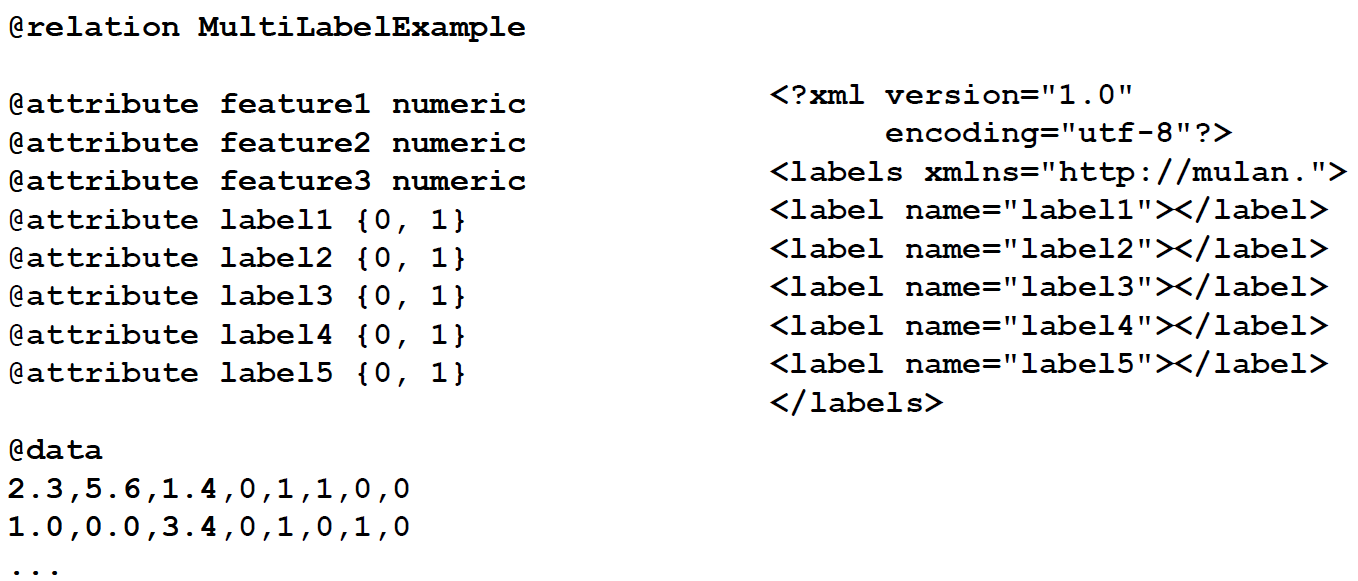
\includegraphics[width=0.45\linewidth]{pic1.png}}
    \label{1a}\hfill
	  \subfloat[b]{
        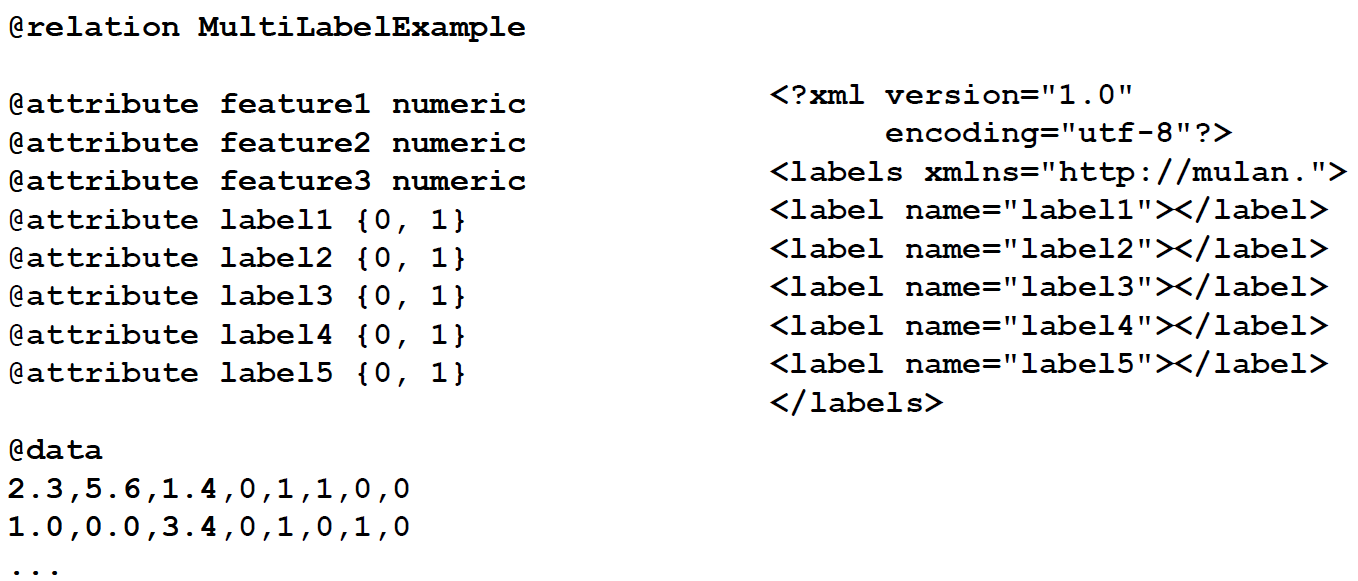
\includegraphics[width=0.45\linewidth]{pic1.png}}
    \label{1b}\\
	  \subfloat[c]{
        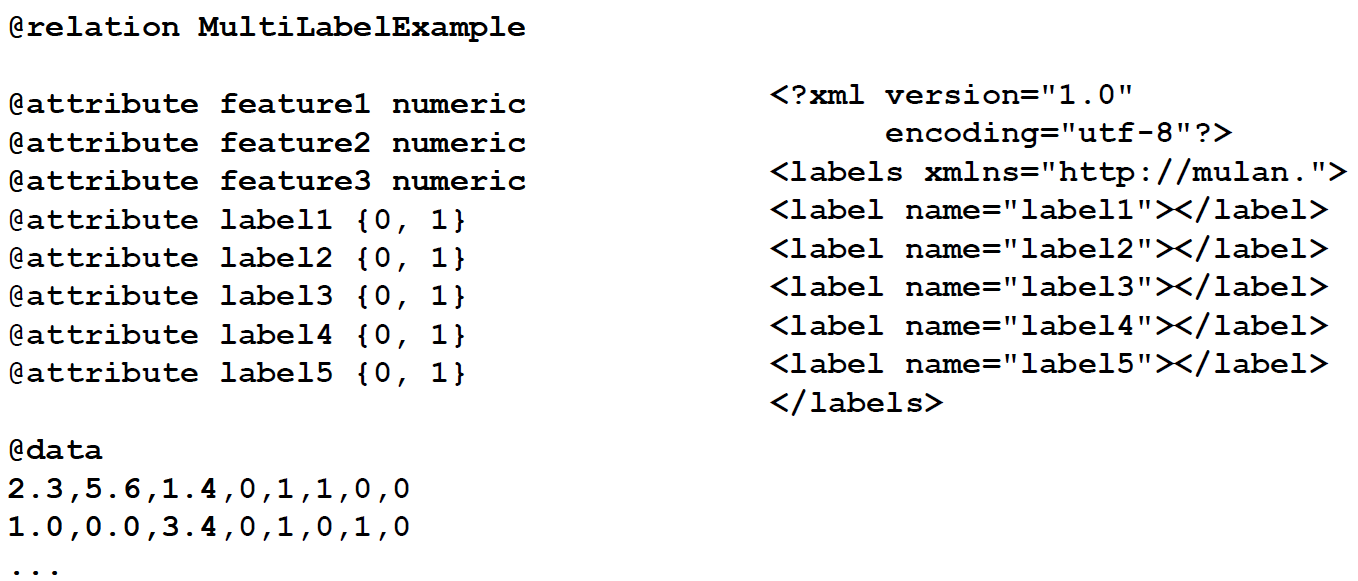
\includegraphics[width=0.45\linewidth]{pic1.png}}
    \label{1c}\hfill
	  \subfloat[d]{
        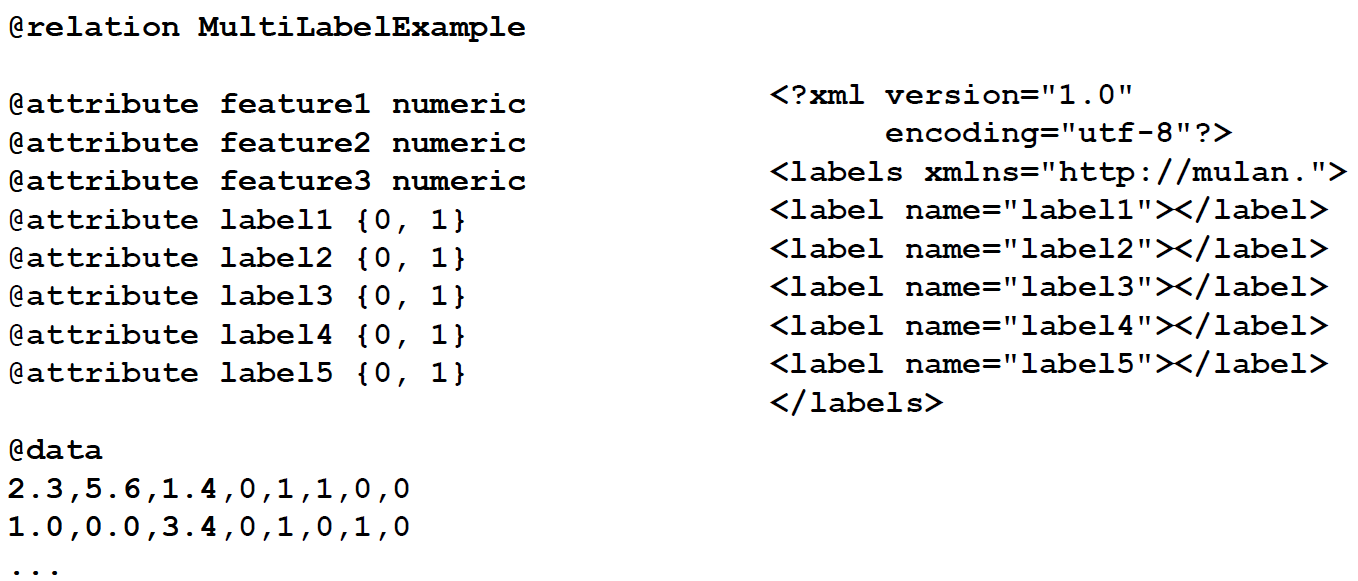
\includegraphics[width=0.45\linewidth]{pic1.png}}
     \label{1d} 
	  \caption{ between objects in the multi-label images.}
	  \label{fig1} 
	\end{figure*}
\lipsum[1-5]
\lipsum[1-3]

\bibliographystyle{IEEEtran}
\bibliography{ref}

\end{document}